%
% CMPT 454: Database Systems II - A Course Overview
% Section: Data Storage Architecture
%
% Author: Jeffrey Leung
%

\section{Data Storage}
	\label{sec:data-storage-architecture}
\begin{easylist}

& DBMS manages disk space and buffer management instead of delegating to the OS
	&& Reason: Needs to support multiple OS platforms and files which span multiple disks

& \textbf{Main memory:} RAM data storage; location where current working data is stored
	&& Data is automatically removed upon power loss
	&& The whole DB is not stored in memory due to high storage cost and volatility

& \textbf{Disk:} Hard drive data storage; location where the main database is stored
	&& Faster than tapes (which are sequential) due to being random access

& Tapes: Infrequent method for archiving older database versions

& \textbf{System catalog:} Database relation which contains information about relations, indices, and views
	&& Relation/file information: Name, structure type, attributes and types, indices, integrity constraints
	&& Index information: Name, structure type, search key
	&& View information: Name, definition

\end{easylist}
\subsection{Physical Disk Components}
	\label{subsec:physical-disk-components}
\begin{easylist}

\begin{figure}[!htb]
	\centering
	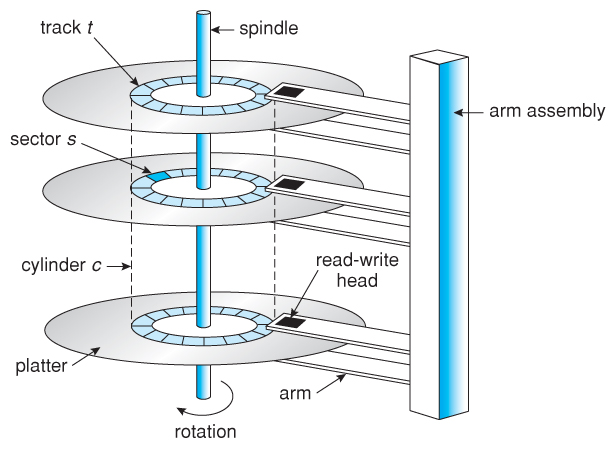
\includegraphics[width=.8\linewidth]{data-storage-architecture/arm-assembly-diagram}
	\caption{Arm Assembly Diagram}
	\label{img:arm-assembly-diagram}
\end{figure}

& Arm: Component which moves along platters to read data
	&& Head: Component on an arm which reads data

& Platter: Single double-sided physical plate in a hard drive which rotates
	&& \textbf{Track:} Circular section of data on a platter
		&&& \textbf{Cylinder:} Set of circular tracks vertically adjacent across all platters
	&& \textbf{Sector:} Pie-shaped section of a platter, from the outer edge to the middle
		&&& \textbf{Track sector:} Section of a track in a specific sector

& Read/write movements:
	&& Seek time: High-cost time required to position an arm on a disk
	&& Rotational delay: High-cost time required to rotate a platter to a position
	&& Transfer time: Low-cost time to read data from the disk with the head

& I/O operations are high-cost because they need mechanical components
	&& Read: Transfer of data from disk to main memory
	&& Write: Transfer of data from main memory to disk

\end{easylist}
\subsection{Data Pages and Frames}
	\label{subsec:data-pages-and-frames}
\begin{easylist}
	
& \textbf{Page:} Fixed-size block of data
	&& Files are stored as a collection of pages
	&& On physical disk:
		&&& Consists of a contiguous set of sectors on a single track
		&&& Smallest possible unit of data retrieval
		&&& Location impacts performance
		&&& Page ID is uniquely identified by $(b, t, c, d)$: Block $b$ of track $t$ of cylinder $c$ of disk $d$
	
	&& \textbf{Next page concept:} Sequential ordering of pages on the disk to minimize access time
		&&& Process:
			&&&& Next page on the same track
			&&&& Next page on the same cylinder
			&&&& Next page on the adjacent cylinder 
		&&& Minimizes seek and rotational delay

	&& \textbf{Sequential scan:} Reading of multiple disk pages sequentially
		&&& Allows pre-fetching of several pages at a time
	&& Fragmentation: Deleted data leaves unallocated spaces of varying sizes on a disk
		&&& Means that files are not guaranteed to be stored sequentially on disk


& \textbf{Frame:} Fixed-size space for data in physical memory
	&& For any read/write operation, the target data must first be in memory (i.e. the page containing the data must be allocated in a frame)

	&& \textbf{Dirty frame:} Frame which has unsaved modifications
		&&& A bit is used to mark dirty status upon modification
	&& \textbf{Pinned frame:} Frame which is currently in use and cannot be replaced
		&&& \textbf{Pin count:} Number of currently active users of a page

\end{easylist}
\subsection{Accessing Data Pages}
	\label{subsec:accessing-data-pages}
\begin{easylist}

& \textbf{Page fault:} Operation when a page is required but not currently in memory
	&& If a page fault occurs:
		&&& A non-pinned frame is selected
		&&& If the frame is dirty, it is saved to the disk
		&&& The new frame replaces the old frame
		&&& The new frame is pinned
		&&& The lookup table is updated
		&&& The address of the new frame is returned

& Access pattern: Pattern by which data pages are requested for access
	&& \textbf{Sequential flooding:} Data page access pattern where each page request is for a new page
& Replacement policy: Strategy which determines which frames are kept in memory or removed
	&& Different policies are optimized for different access patterns
	&& Examples: First-in-first-out (FIFO), least-recently-used (LRU), most-recently-used (MRU)

\clearpage

\end{easylist}
\subsection{Storing Records on a Page: Fixed-Length}
	\label{subsec:storing-records-on-a-page-fixed-length}
\begin{easylist}

& Introduction to records and fields:
	
	&& \textbf{Field:} Section of a record; represents a single primitive datatype
		&&&& Abbreviation: $Fx$ where $x$ is the number of the given field in order
		&&&& Abbreviation of the length of a field: $Lx$ where $x$ is the number of the given field in order

	&& \textbf{Record:} Section of a file; represents a unique data entity
		&&& Base address ($B$): Beginning location of a record on its page
		&&& Length of a record equals the sum of the length of all its fields
			&&&& Calculation: $L = \sum Li$
			&&&& Location of the $i^{\textrm{th}}$ record: $B = (i-1) \times L$
		&&& \textbf{Slot:} Location of a record on a page
		&&& \textbf{Record ID (RID):} Location of a record
			&&&& Identified by (page ID, slot \#)

& \textbf{Fixed-length record format:} Data page format where all records have the same types and numbers of fields
	&& Length of records are identical
	&& Diagram: See figure~\ref{img:record-fixed}
	
	\begin{figure}[!htb]
		\centering
		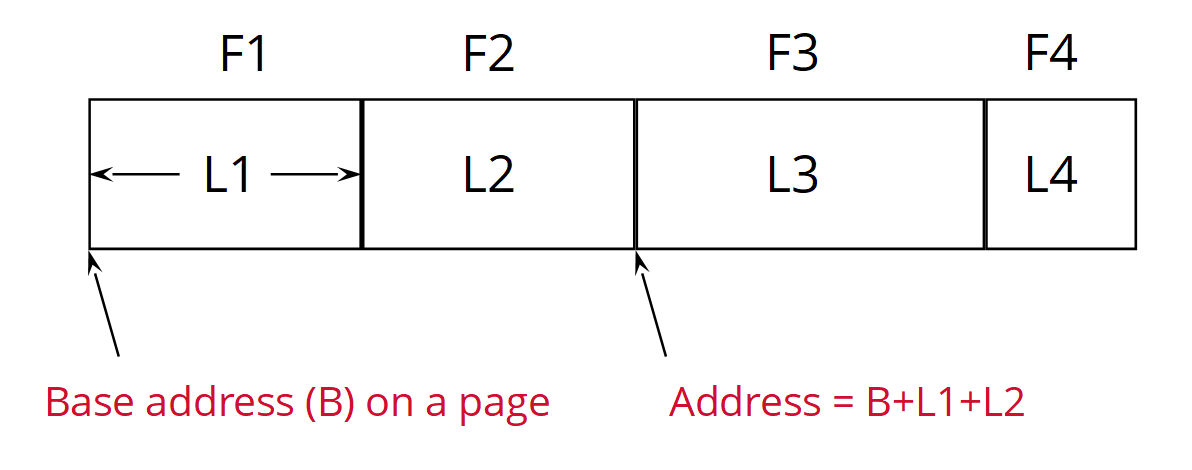
\includegraphics[width=.8\linewidth]{data-storage-architecture/record-fixed}
		\caption{Fixed-length record format}
		\label{img:record-fixed}
	\end{figure}


& \textbf{Packed page:} Fixed-length record format where free space is always organized contiguously
	&& Diagram: See figure~\ref{img:record-fixed-packed}
	
	\begin{figure}[!htb]
		\centering
		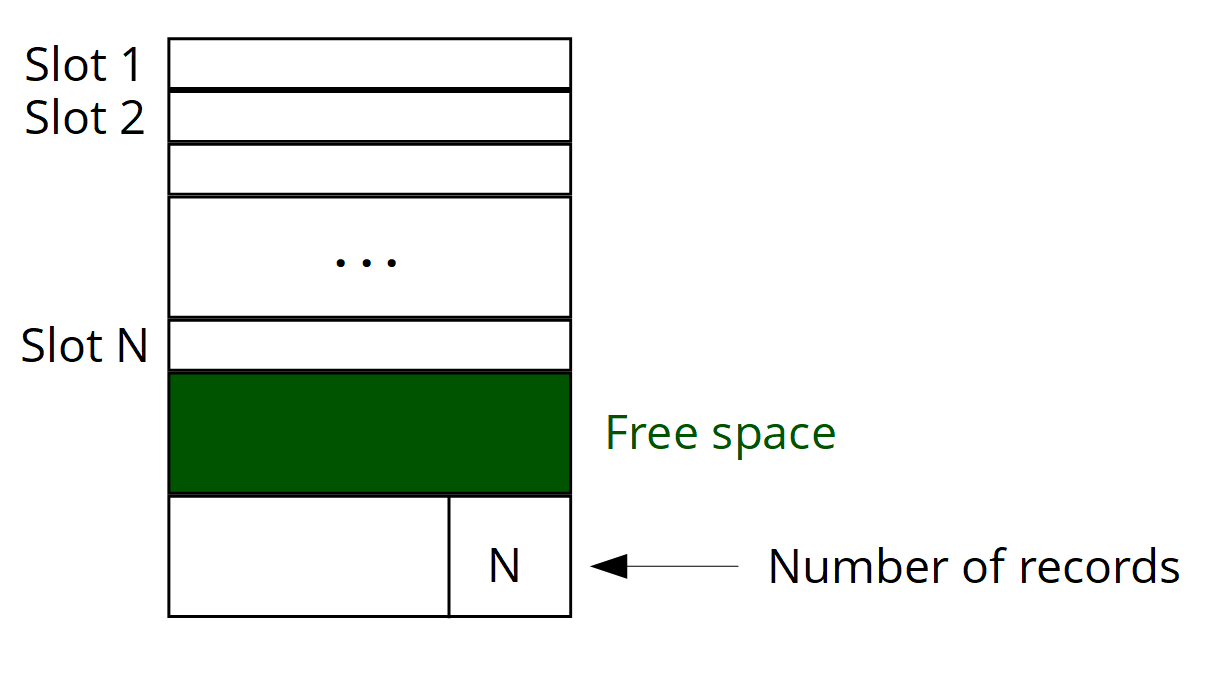
\includegraphics[width=.8\linewidth]{data-storage-architecture/record-fixed-packed}
		\caption{Packed page with fixed-length ecords}
		\label{img:record-fixed-packed}
	\end{figure}
	
	&& Contains a value with the number of currently allocated records
	&& Record addition: Allocate a slot from the start of free space
	&& Record deletion: De-allocate the slot, move the following data up to be contiguous
	&& Incurs no operation overhead as the data is in memory

& \textbf{Unpacked page:} Fixed-length record format where free space is not contiguous
	&& Diagram: See figure~\ref{img:record-fixed-unpacked}
	
	\begin{figure}[!htb]
		\centering
		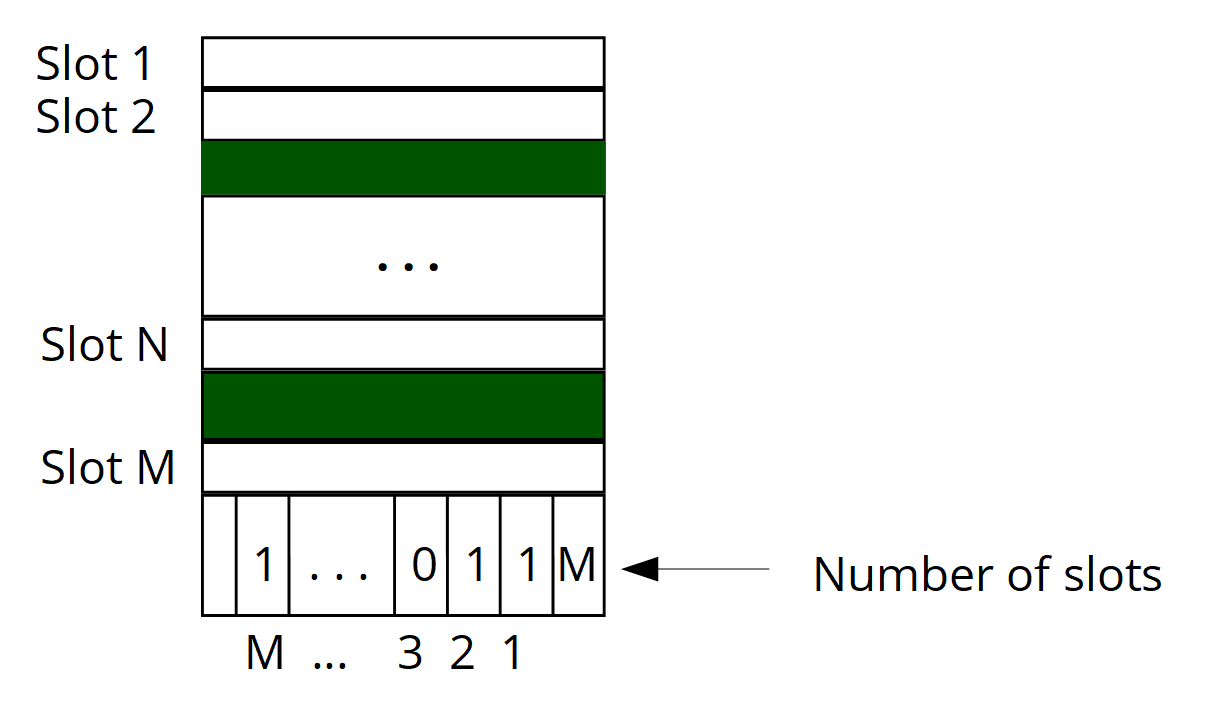
\includegraphics[width=.8\linewidth]{data-storage-architecture/record-fixed-unpacked}
		\caption{Unpacked page with fixed-length records}
		\label{img:record-fixed-unpacked}
	\end{figure}
	
	&& Contains a value with the number of currently unallocated records
	&& Free space is tracked by a bitmap at the end of the page, which represents whether a slot is allocated or free
	&& Record addition: Check the bitmap to find a free slot to allocate
	&& Record deletion: De-allocate the slot in the bitmap
	&& Incurs no operation overhead as the data is in memory

\end{easylist}
\subsection{Storing Records on a Page: Variable-Length}
	\label{subsec:storing-records-on-a-page-variable-length}
\begin{easylist}

& \textbf{Variable-length record format:} Record format where each record on a page may have differing fields
	&& Records contain a value representing the number of fields

	&& \textbf{Fixed-fields variable-length record format:} Data page format where, for all records, the number of fields cannot dynamically change (but the records may have differing fields)
		&&& Diagram: See figure~\ref{img:record-variable-fixed}
	
		\begin{figure}[!htb]
			\centering
			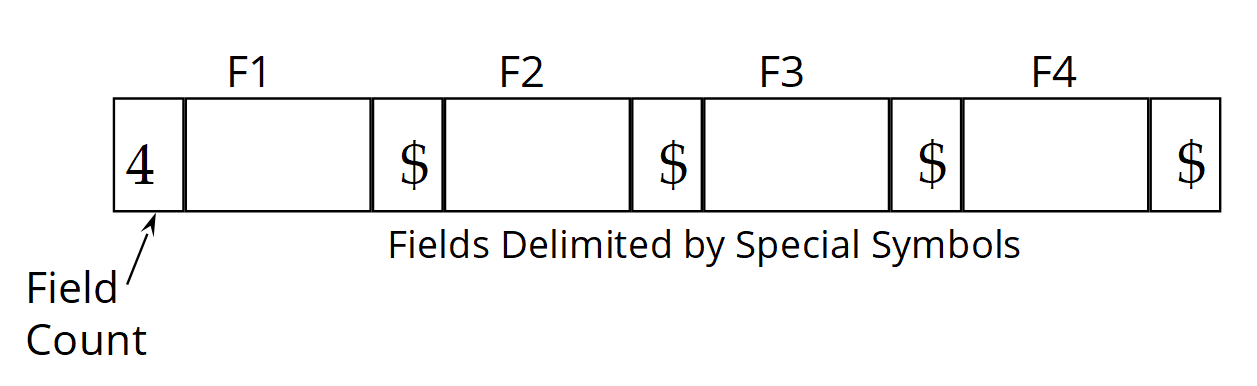
\includegraphics[width=.8\linewidth]{data-storage-architecture/record-variable-fixed}
			\caption{Variable-length records with fixed fields}
			\label{img:record-variable-fixed}
		\end{figure}
	
		&&& Fields are delimited by unique symbols
		&&& Access method: Sequential scan from beginning to end
	
	&& \textbf{Variable-fields variable-length record format:} Data page format where, for all records, the number of fields cannot dynamically change (but the records may have differing fields)
		&&& Diagram: See figure~\ref{img:record-variable-variable}
	
		\begin{figure}[!htb]
			\centering
			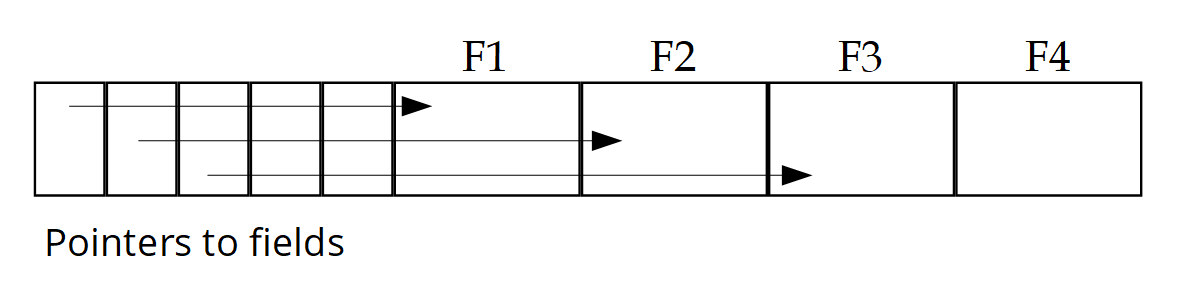
\includegraphics[width=.8\linewidth]{data-storage-architecture/record-variable-variable}
			\caption{Variable-length records with variable fields}
			\label{img:record-variable-variable}
		\end{figure}
		
		&&& Record contains a set of pointers to each field
			&&&& Incurs a space overhead
		&&& Access method: Directly from the set of pointers
		&&& Allows easy nullable storage


& Storage of variable-length records on a page:
	&& Diagram: See figure~\ref{img:record-variable-page}
	
	\begin{figure}[!htb]
		\centering
		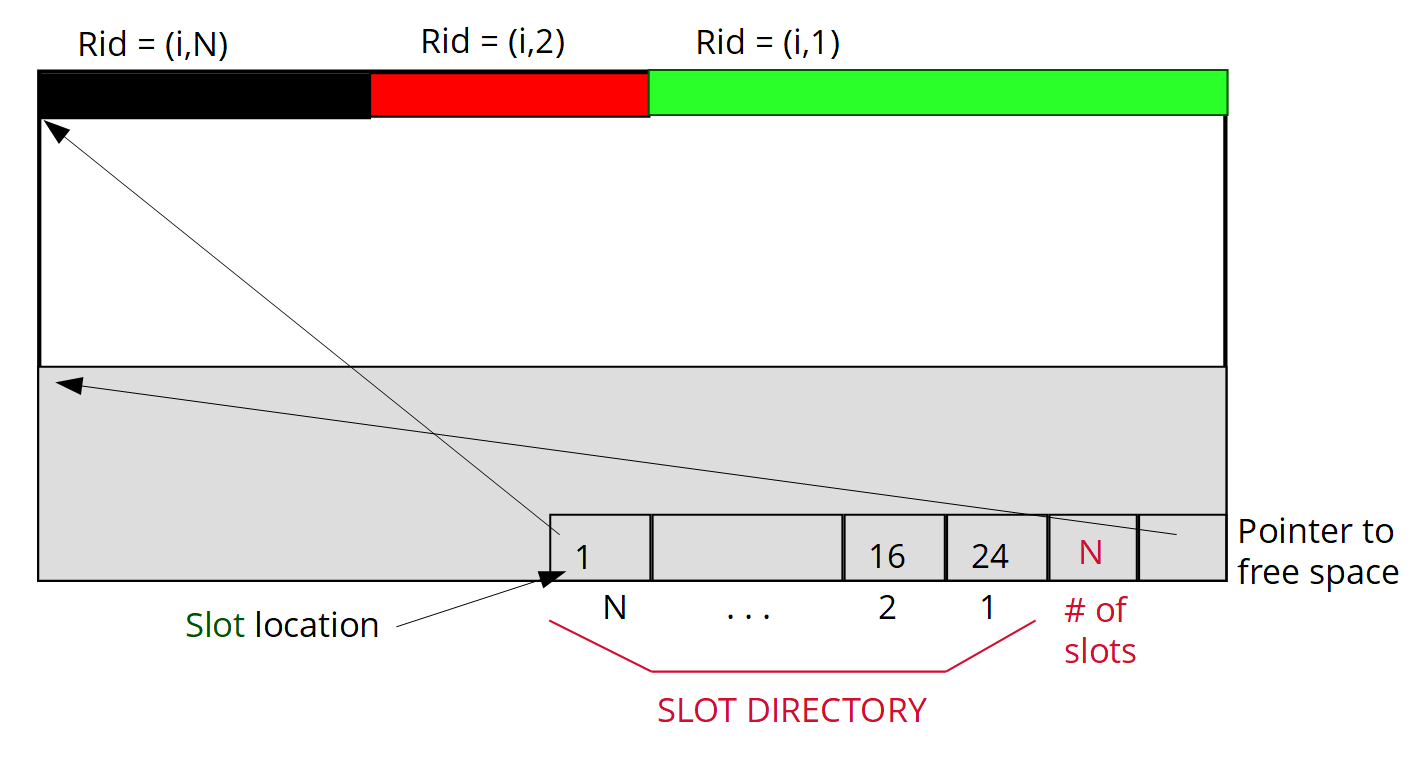
\includegraphics[width=.8\linewidth]{data-storage-architecture/record-variable-page}
		\caption{Page of variable-length records}
		\label{img:record-variable-page}
	\end{figure}
	
	&& Page contains a:
		&&& Value with the number of currently allocated slots
		&&& Pointer to first available free space
		&&& Slot directory (at the end of the page) with the starting location of each records
	&& Records are allocated by filling the next free space, and linking to it with any free slot in the directory



\end{easylist}
\clearpage













